\section{Comparaison avec la photo en saturation plus
élevée}\label{comparaison-avec-la-photo-en-saturation-plus-uxe9levuxe9e}

\begin{figure}[htbp]
\centering
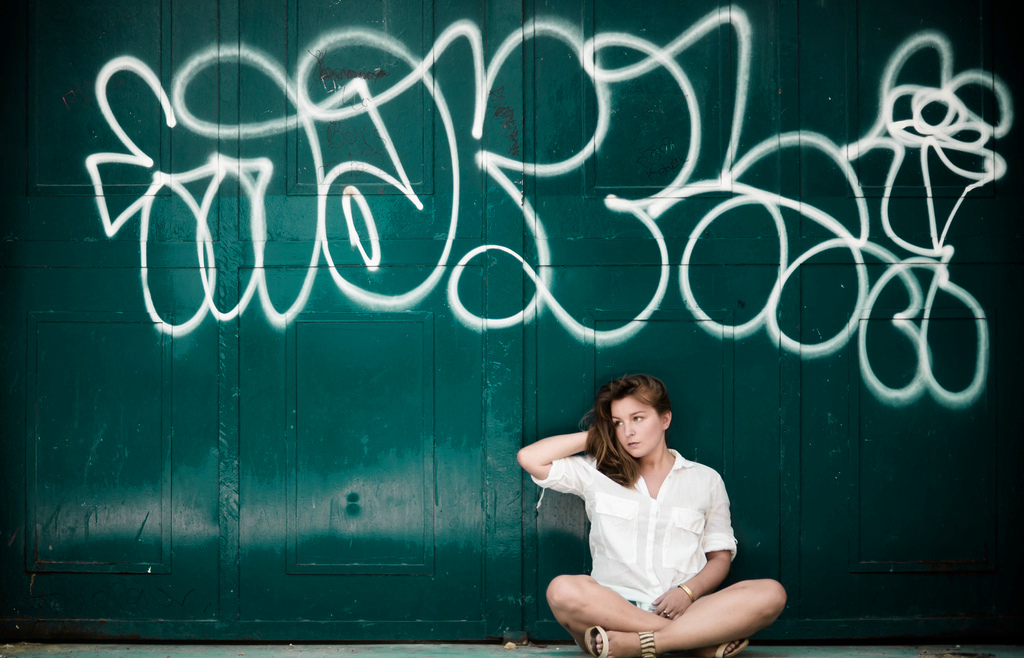
\includegraphics{../../photos/saturate.jpg}
\caption{Photo en saturation élevée}
\end{figure}

\begin{table}[htbp]
\centering
\begin{tabular}{llr}
\bfseries Formes &
\bfseries Bhattacharyya (\%)%
\DTLforeach*[\DTLiseq{\fichier}{photos/saturation.jpg}]{valeurs}{%
\fichier=Fichier, \formes=Formes,\bhatta=Bhattacharyya}{%
\\
\formes & \bhatta}
\end{tabular}
\end{table}

On observe avec la comparaison de cette photo saturée que selon nos
critères, ces deux photos se ressemblent ($0.94 \%$ de différence pour la
colorimétrie avec la distance de Bhattacharyya et $0.51 \%$ de différence
pour les formes avec l'application du filtre de Sobel).\\ En effet, les
couleurs sont légèrement moins ternes sur la photo saturée et les quelques
contours décelés au filtre de Sobel sont dû aux points de lumière qui sont plus
visibles et détourés.
